\documentclass[12pt]{report}
\usepackage[utf8]{inputenc}
\usepackage[margin=1.2in]{geometry}
\usepackage{graphicx}
\usepackage{float}
\usepackage{subcaption}
\usepackage{amsmath}
\usepackage{amssymb}
\usepackage{ulem}
\usepackage{bm}
\usepackage{framed}
\usepackage{xcolor}
\usepackage{ragged2e}
\usepackage{color}
\usepackage{soul}
\usepackage{cancel}
\graphicspath{ {images/} }
\setlength{\parskip}{1em}
\allowdisplaybreaks


\usepackage{titling}
\newcommand{\subtitle}[1]{%
	\posttitle{%
		\par\end{center}
	\begin{center}\large#1\end{center}
	\vskip0.5em}%
}

\newenvironment{blueframed}[1][blue]
{\def\FrameCommand{\fboxsep=\FrameSep\fcolorbox{#1}{white}}%
\MakeFramed {\advance\hsize-\width \FrameRestore}}
{\endMakeFramed}

\newenvironment{spmatrix}[1]
{\def\mysubscript{#1}\mathop\bgroup\begin{bmatrix}}
{\end{bmatrix}\egroup_{\textstyle\mathstrut\mysubscript}}

\title{Tutorial 6}
\subtitle
{
\textbf{keywords}: hypothesis testing, t-test, test statistic, critical value, confidence intervals, R-squared, interpretation of coefficients, multiple linear regression, omitted variable bias

\textbf{estimated reading time}: 33 minutes
}
\author{Quang Bui}
\date{April 9, 2018}

\begin{document}

\maketitle

\section*{Question 1}
\noindent \textcolor{red}{A sample of 25 employees was taken. Each employee was asked to assess his own job satisfaction ($X$) on a scale from 1 to 10. The number of days ($Y$) an employee was absent from work was also registered. Fitting a linear regression model based on least squares method gave the sample regression line, $$\hat{Y} = 13.6 - 1.2X$$ Also found were: $$\bar{X} = 6.0 \quad \sum_{i=1}^{n}(X_I - \bar{X})=130 \quad SSR = 80.6 \quad ESS = 186.9$$}

\noindent \textcolor{red}{(a) Test at the 1\% level that job satisfaction has no effect on absenteeism using the t-test based on the sample slope estimate.}

\noindent For the simple linear regression model of absenteeism $(Y)$, $$Y = \beta_0 + \beta_1 X + u$$ $\beta_1$ measures the true effect of job satisfaction on absenteeism (not holding any variable(s) constant). 

\noindent If job satisfaction does not have a true effect on absenteeism then, $$\beta_1 = 0$$ but if it does,  $$\beta_1 \neq 0$$ After we estimate our model, $$\hat{Y} = 13.6 - 1.2X$$ we can perform this hypothesis test.

\noindent \textbf{State the null and alternative hypothesis}
\vspace{15mm}

\noindent \textbf{The test statistic and its distribution under $H_0$}

\newpage
\noindent \textbf{Calculate the test statistic}
\vspace{60mm}



\noindent \textbf{Critical value and rejection region}
\vspace{40mm}

\begin{figure}[H]
	\centering
	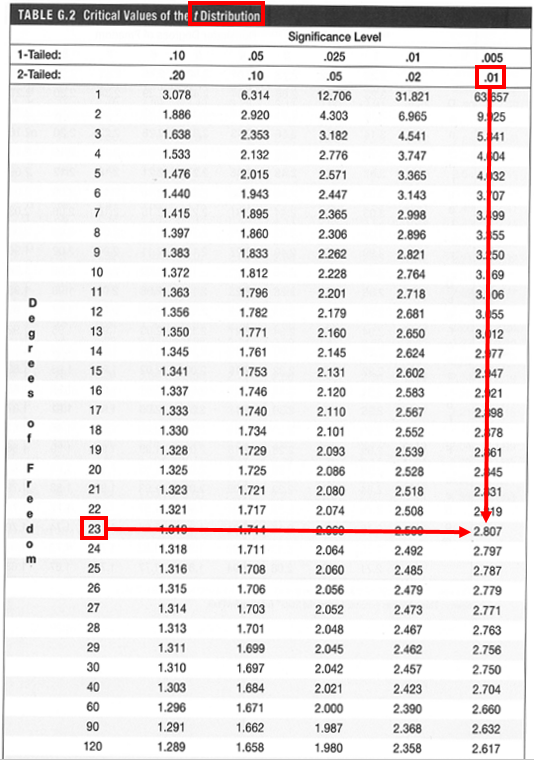
\includegraphics{tute6_q1_1}
\end{figure}
\vspace{-\baselineskip}
\noindent From the statistics table: \begin{align*}
+t_{crit} &=  \\
-t_{crit} &= 
\end{align*}
\noindent To obtain the critical value using EViews,
$$Command\ window:\ =@qtdist(0.995,23)$$
\begin{figure}[H]
	\centering
	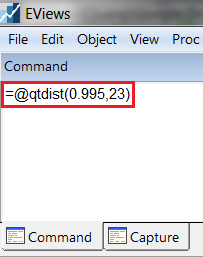
\includegraphics{tute6_q1_2}
\end{figure}
\vspace{-\baselineskip}\centering $(press\ Enter\ to\ execute)$
\justify and the value appears in the bottom left corner,
\begin{figure}[H]
	\centering
	
\includegraphics{tute6_q1_3}
\end{figure}
\vspace{-\baselineskip}
\noindent From EViews: \begin{align*}
+t_{crit} &= t_{23,0.005} = 2.807 \\
-t_{crit} &= t_{23,0.005} = -2.807
\end{align*}
\noindent For a two-sided t-test, we reject $H_0$ if,
$$t_{calc} > +t_{crit}$$
$$or$$
$$t_{calc} < -t_{crit}$$
\noindent \textbf{Conclusion}
\vspace{20mm}

\noindent \textcolor{red}{(b) Compute the coefficient of determination and comment on it.}


\newpage
\section*{Question 2}
\noindent \textcolor{red}{Suppose that $(y_i,x_i)$ satisfy the Classical Linear Model assumptions. A random sample of size $n=250$ is drawn and yields,
\begin{align*}
	\hat{y}_i &= \underset{(3.1)}{5.4} + \underset{(1.5)}{3.2}x_i \quad i=1,2,\dots,n \\
	R^2 &= 0.26 \quad SER\ (Standard\ Error\ of\ Regression) = 6.2
\end{align*} (a) Test $H_0: \beta_1 = 0$ vs $H_1: \beta_1 \neq 0$ at the 5\% level where $\beta_1$ is the slope coefficient in the above regression.}

\noindent For the simple linear regression model of $y$, $$y = \beta_0 + \beta_1 x + u$$ $\beta_1$ measures the true impact that $x$ has on $y$ (not holding any variable(s) constant). 

\noindent If $x$ does not have a true significant impact on $y$ then, $$\beta_1 = 0$$ but if it does,  $$\beta_1 \neq 0$$ After we estimate our model, $$\hat{y} = \underset{(3.1)}{5.4} + \underset{(1.5)}{3.2}x$$ we can perform this hypothesis test.

\noindent \textbf{State the null and alternative hypothesis}
\begin{align*}
H_0&: \beta_1 = 0 \\
H_1&: \beta_1 \neq 0
\end{align*}
\noindent \textbf{The test statistic and its distribution under $H_0$}
\begin{align*}
t &= \dfrac{\hat{\beta}_1 - \beta_1}{se(\hat{\beta}_1)} = \dfrac{\hat{\beta}_1 - 0}{se(\hat{\beta}_1)} = \dfrac{\hat{\beta}_1}{se(\hat{\beta}_1)} \sim t_{n-k-1} \quad under\ H_0 \\
n &= sample\ size = 250 \\
k &= no.\ of\ regressors\ in\ the\ model = 1 \\
d.o.f &= n-k-1=248
\end{align*}
\noindent \textbf{Calculate the test statistic}
$$t_{calc} = \dfrac{\hat{\beta}_1}{se(\hat{\beta}_1)} = \dfrac{3.2}{1.5} = 2.1333$$
\noindent \textbf{Critical value and rejection region}

\noindent $5\%\ significance\ level\ \therefore \alpha = 0.05$, two-sided t-test

\noindent Since we are performing a t-test, the critical value(s) (which bounds the rejection region) come from a t-distribution. The t-distribution of interest in this hypothesis test, is one with $degrees\ of\ freedom\ = n - k - 1 = 250 - 2 = 248$. Since $d.o.f = 248$ is not in the statistics table, we take a conservative approach and choose the closest available degrees of freedom less than 248 i.e. $d.o.f=120$. 
\begin{figure}[H]
	\centering
	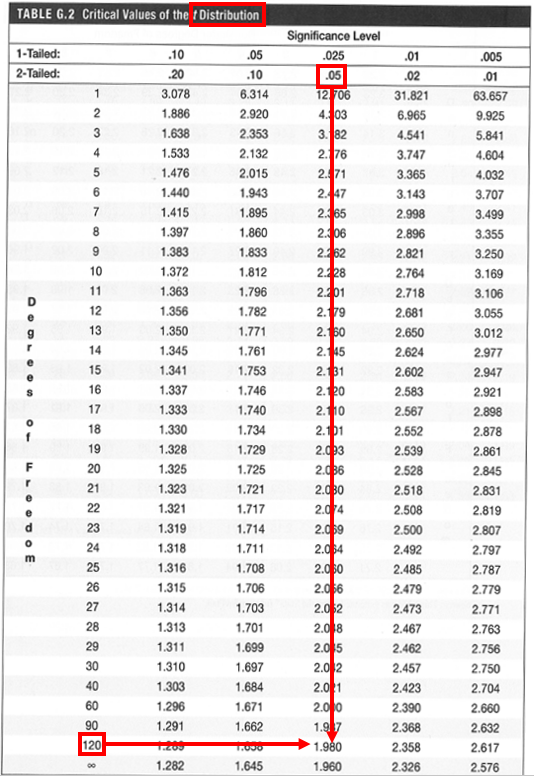
\includegraphics{tute6_q2_1}
\end{figure}
\vspace{-\baselineskip}
\noindent From the statistics table: \begin{align*}
	+t_{crit} &= 1.980 \\
	-t_{crit} &= -1.980
\end{align*}
\noindent To obtain the critical value using EViews,
$$Command\ window:\ =@qtdist(0.975,248)$$
\begin{figure}[H]
	\centering
	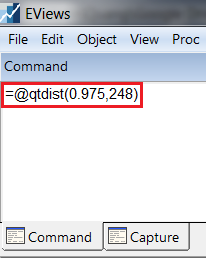
\includegraphics{tute6_q2_2}
\end{figure}
\vspace{-\baselineskip}\centering $(press\ Enter\ to\ execute)$
\justify and the value appears in the bottom left corner,
\begin{figure}[H]
	\centering
	
\includegraphics{tute6_q2_3}
\end{figure}
\vspace{-\baselineskip}
\noindent From EViews: \begin{align*}
+t_{crit} &= t_{248,0.975} = 1.970 \\
-t_{crit} &= t_{248,0.025} = -1.970
\end{align*}
\noindent For a two-sided t-test, we reject $H_0$ if,
$$t_{calc} > +t_{crit}$$
$$or$$
$$t_{calc} < -t_{crit}$$
\noindent \textbf{Conclusion}

\noindent Since $t_{calc} = 2.1333 > +t_{crit} = 1.970$, we reject the null at the 5\% significance level and conclude that there is sufficient evidence from our sample to suggest that $x$ has a statistically significant impact on $y$.

\newpage
\noindent \textcolor{red}{(b) Construct a 95\% confidence interval for $\beta_1$}
\vspace{40mm}

\noindent \textcolor{red}{(c) Suppose that you learn that $y_i$ and $x_i$ are independent. Would you be surprised? Explain.}
\vspace{60mm}

\noindent \textcolor{red}{(d) Suppose that you learn that $y_i$ and $x_i$ are independent and many samples of $n=250$ are drawn, regressions estimated, and (a) and (b) answered. In what fraction of the samples would $H_0$ from (a) be rejected? In what fraction of samples would the value $\beta_1 = 0$ be included in the confidence interval from (b)?}

\noindent The significance level, $\alpha$, is the probability of rejecting the null hypothesis when it is true. Since we set $\alpha = 0.05$, the probability of rejecting $H_0: \beta_1=0$ when it is true i.e. $x_i$ has no true impact on $y_i$ is 0.05.

\noindent Therefore, given that $x_i$ does not help to explain $y_i$ (because they are independent), we would reject $H_0: \beta_1=0$ in 5\% of the samples.

\noindent The true value of $\beta_1$ will lie in 95\% of the confidence intervals. If we learn that $y_i$ and $x_i$ are independent, then the true value of $\beta_1$ is $0$, so $\beta_1 = 0$ would lie in 95\% of the confidence intervals.

\newpage
\section*{Question 3}
\noindent \textcolor{red}{File $401KSUBS.wf1$ contains information on net financial wealth ($nettfa$), age of the survey respondent ($age$), annual family income ($inc$), family size ($fsize$), and participation in certain pension plans for people in the United States. The wealth and income variables are both recorded in thousands of dollars.}

\noindent \textcolor{red}{(a) How many single-person households are there in the data set?}

\noindent We need to change our sample to include only single-person households. In EViews,
click on $Sample$ and type $fsize=1$ in the $IF\ condition$ dialog box,
\begin{figure}[H]
	\centering
	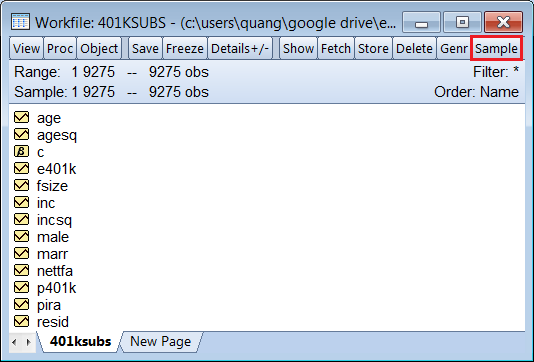
\includegraphics{tute6_q3_1}
\end{figure}
\vspace{-\baselineskip}
\begin{figure}[H]
	\centering
	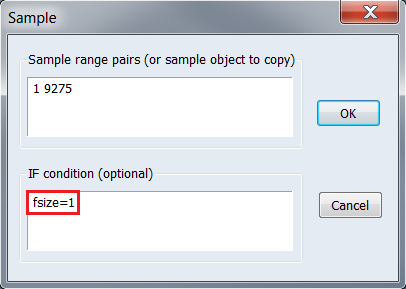
\includegraphics{tute6_q3_2}
\end{figure}
\vspace{-\baselineskip}
\noindent This tells EViews to change the current working sample, to a sample of only single-person households,
\begin{figure}[H]
	\centering
	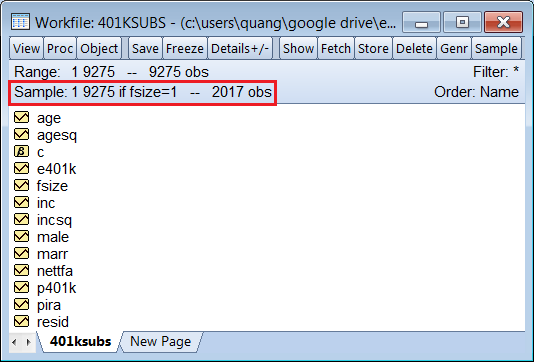
\includegraphics{tute6_q3_3}
\end{figure}
\vspace{-\baselineskip}
\noindent \textcolor{red}{Using the data only for single-person households, estimate the model $$nettfa_i = \beta_0 +\beta_1inc_i + \beta_2age_i + u_i \quad i=1,2,\dots,2017$$ Report the estimated equation (including standard errors of coefficients). Interpret the slope coefficients. Are there any surprises in the slope estimates.}

\noindent To estimate an model from the Command window,
$$ls\ nettfa\ c\ inc\ age$$
\begin{figure}[H]
	\centering
	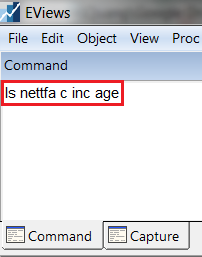
\includegraphics{tute6_q3_4}
\end{figure}
\vspace{-\baselineskip}\centering $(press\ Enter\ to\ execute\ code)$
\justify 
%%%%%%%%%% TABLE OBJECT %%%%%%%%%%
\begin{table}[H]
	\centering
	\begin{tabular}{lrrrr}
		\multicolumn{3}{l}{Dependent Variable: NETTFA}&\multicolumn{1}{c}{}&\multicolumn{1}{c}{}\\
		\multicolumn{3}{l}{Method: Least Squares}&\multicolumn{1}{c}{}&\multicolumn{1}{c}{}\\
		\multicolumn{3}{l}{Date: 04/07/18   Time: 18:24}&\multicolumn{1}{c}{}&\multicolumn{1}{c}{}\\
		\multicolumn{3}{l}{Sample: 1 9275 IF FSIZE=1}&\multicolumn{1}{c}{}&\multicolumn{1}{c}{}\\
		\multicolumn{3}{l}{Included observations: 2017}&\multicolumn{1}{c}{}&\multicolumn{1}{c}{}\\
		[4.5pt] \hline \\ [-4.5pt]
		\multicolumn{1}{c}{Variable}&\multicolumn{1}{r}{Coefficient}&\multicolumn{1}{r}{Std. Error}&\multicolumn{1}{r}{t-Statistic}&\multicolumn{1}{r}{Prob.}\\
		[4.5pt] \hline \\ [-4.5pt]
		\multicolumn{1}{c}{C}&\multicolumn{1}{r}{$-43.03981$}&\multicolumn{1}{r}{$4.080393$}&\multicolumn{1}{r}{$-10.54796$}&\multicolumn{1}{r}{$0.0000$}\\
		\multicolumn{1}{c}{INC}&\multicolumn{1}{r}{$0.799317$}&\multicolumn{1}{r}{$0.059731$}&\multicolumn{1}{r}{$13.38200$}&\multicolumn{1}{r}{$0.0000$}\\
		\multicolumn{1}{c}{AGE}&\multicolumn{1}{r}{$0.842656$}&\multicolumn{1}{r}{$0.092017$}&\multicolumn{1}{r}{$9.157631$}&\multicolumn{1}{r}{$0.0000$}\\
		[4.5pt] \hline \\ [-4.5pt]
		\multicolumn{1}{l}{R-squared}&\multicolumn{1}{r}{$0.119343$}&\multicolumn{2}{l}{Mean dependent var}&\multicolumn{1}{r}{$13.59498$}\\
		\multicolumn{1}{l}{Adjusted R-squared}&\multicolumn{1}{r}{$0.118469$}&\multicolumn{2}{l}{S.D. dependent var}&\multicolumn{1}{r}{$47.59058$}\\
		\multicolumn{1}{l}{S.E. of regression}&\multicolumn{1}{r}{$44.68275$}&\multicolumn{2}{l}{Akaike info criterion}&\multicolumn{1}{r}{$10.43854$}\\
		\multicolumn{1}{l}{Sum squared resid}&\multicolumn{1}{r}{$4021048.$}&\multicolumn{2}{l}{Schwarz criterion}&\multicolumn{1}{r}{$10.44688$}\\
		\multicolumn{1}{l}{Log likelihood}&\multicolumn{1}{r}{$-10524.27$}&\multicolumn{2}{l}{Hannan-Quinn criter.}&\multicolumn{1}{r}{$10.44160$}\\
		\multicolumn{1}{l}{F-statistic}&\multicolumn{1}{r}{$136.4648$}&\multicolumn{2}{l}{Durbin-Watson stat}&\multicolumn{1}{r}{$1.959509$}\\
		\multicolumn{1}{l}{Prob(F-statistic)}&\multicolumn{1}{r}{$0.000000$}&\multicolumn{1}{c}{}&\multicolumn{1}{c}{}&\multicolumn{1}{c}{}\\
		[4.5pt] \hline \\ [-4.5pt]
	\end{tabular}
	\caption{Regression output of $nettfa$ on a constant, $inc$, and $age$.}
	%\label{tab:}
\end{table}
\vspace{-\baselineskip}
\centering $\widehat{nettfa} = -\underset{(4.0804)}{43.0398} + \underset{(0.0597)}{0.7993}inc + \underset{(0.0920)}{0.8427}age$

\justify \noindent Interpretations of the estimated coefficients:

\noindent $\hat{\beta}_1 = 0.7993$ - The model estimates that for an additional \$1,000 in income, net financial wealth is predicted to increase by approximately \$800, on average, holding the age of the individual constant. ($nettfa$ and $inc$ are measured in \$'000.)

\noindent $\hat{\beta}_2 = 0.8427$ - The model estimates that if a person ages by 1 year, his/her net financial wealth is predicted to increase by approximately \$843, on average, holding income constant. ($nettfa$ is measured in \$'000.)

\noindent \textcolor{red}{(c) Does the intercept in (b) have an interesting meaning? Explain.}

\noindent $\hat{\beta}_0 = -43.0398$. The estimated intercept coefficient represents the predicted net financial wealth for an individual aged 0 with no income. The population of interest is single-person households and there are clearly no one with those characteristics in this population.

\newpage
\noindent \textcolor{red}{(d) Test the hypothesis that $H_0: \beta_2 = 1$ against $H_1: \beta_2 < 1$. Do you reject the null hypothesis at the 1\% significance level?}

\noindent We are testing the null hypothesis that aging by one year increases net financial wealth by \$1,000, against the alternative hypothesis that it increases net financial wealth by less than \$1,000. ($nettfa$ is measured in \$'000.)

\noindent \textbf{State the null and alternative hypothesis}
\vspace{20mm}

\noindent \textbf{The test statistic and its distribution under $H_0$}
\vspace{40mm}

\noindent \textbf{Calculate the test statistic}
\vspace{20mm}

\noindent \textbf{Critical value and rejection region}

\noindent $1\%\ significance\ level\ \therefore \alpha = 0.01$, one-sided t-test on the left tail
\begin{figure}[H]
	\centering
	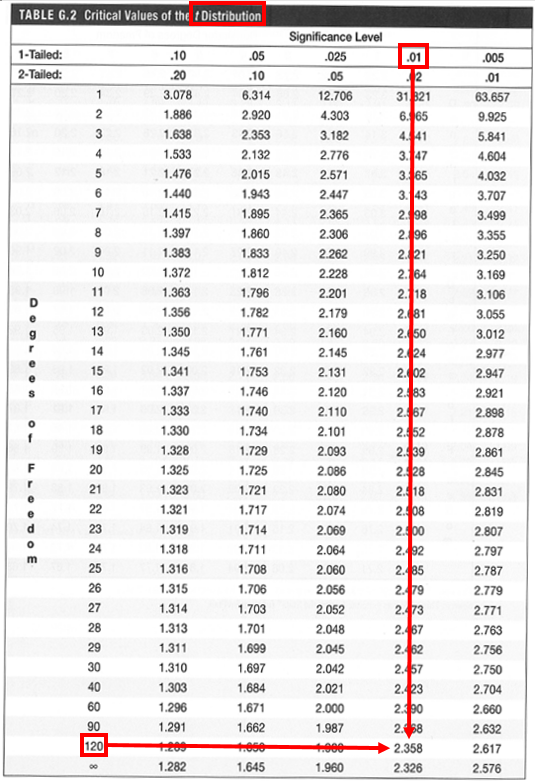
\includegraphics{tute6_q3_5}
\end{figure}
\vspace{-\baselineskip}
\noindent Since we are performing a one-sided t-test on the left tail, where the rejection region lies, we will compare $t_{calc}$ with $-t_{crit}$. From the statistics table: \begin{align*}
-t_{crit} &= -2.358
\end{align*}
\noindent To obtain the critical value using EViews,
$$Command\ window:\ =@qtdist(0.01,2014)$$
\begin{figure}[H]
	\centering
	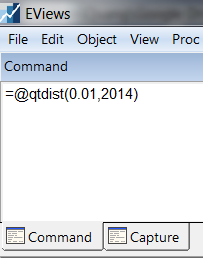
\includegraphics{tute6_q3_6}
\end{figure}
\vspace{-\baselineskip}\centering $(press\ Enter\ to\ execute)$
\justify and the value appears in the bottom left corner,
\begin{figure}[H]
	\centering
	
\includegraphics{tute6_q3_7}
\end{figure}
\vspace{-\baselineskip}
\noindent From EViews: \begin{align*}
-t_{crit} &= -2.3282 
\end{align*}
\noindent For a one-sided t-test on the left tail, we reject $H_0$ if,
$$t_{calc} < -t_{crit}$$
\noindent \textbf{Conclusion}

\noindent Since $t_{calc} = -1.7098 > -t_{crit} = -2.3282$, we do not reject the null at the 1\% significance level and conclude that there is insufficient evidence from our sample to suggest that aging by 1 year increases net financial wealth by less than \$1,000.

\noindent \textcolor{red}{(e) If you omit $age$ from the model and rerun the regression, is the estimated coefficient on $inc$ much different from the estimate in part (b)? Why or why not?}

\noindent The estimated coefficient on $inc$ represents the estimated change in net financial wealth for a unit increase in income, holding age constant. If $age$ were uncorrelated with $inc$, $$\widehat{corr}(age,inc) = 0$$ then whether or not we hold $age$ constant, will not impact the effect of income on net financial wealth. Put differently, if $age$ were strongly correlated with $inc$ or could be a proxy for $inc$, then the effect of income on net financial wealth should change after controlling for the effect of age on net financial wealth constant.

\noindent To obtain the sample correlation coefficient of $age$ and $inc$, $$Quick \to\ Group\ Statistics \to Correlations$$
\begin{figure}[H]
	\centering
	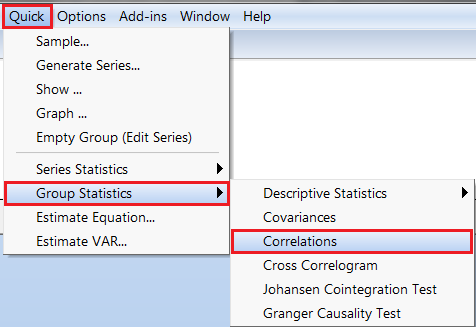
\includegraphics{tute6_q3_8}
\end{figure}
\vspace{-\baselineskip}
\begin{figure}[H]
	\centering
	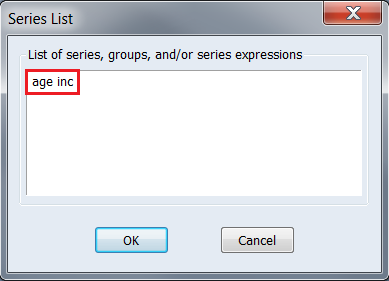
\includegraphics{tute6_q3_9}
\end{figure}
\vspace{-\baselineskip}
%%%%%%%%%% TABLE OBJECT %%%%%%%%%%
\begin{table}[H]
	\centering
	\begin{tabular}{lrr}
		\multicolumn{1}{c}{}&\multicolumn{1}{c}{AGE}&\multicolumn{1}{c}{INC}\\
		\multicolumn{1}{c}{AGE}&\multicolumn{1}{c}{$1.000000$}&\multicolumn{1}{c}{$0.039059$}\\
		\multicolumn{1}{c}{INC}&\multicolumn{1}{c}{$0.039059$}&\multicolumn{1}{c}{$1.000000$}\\
	\end{tabular}
	%\caption{Add your caption here.}
	%\label{tab:}
\end{table} \vspace{-\baselineskip}
\centering $\widehat{corr}(age,inc) = 0.0391$
\justify $age$ and $inc$ have a very weak linear relationship.

\noindent Rerunning the model of $nettfa$ without $age$ using the Command window,
$$Command\ window: ls\ nettfa\ c\ inc$$
\begin{figure}[H]
	\centering
	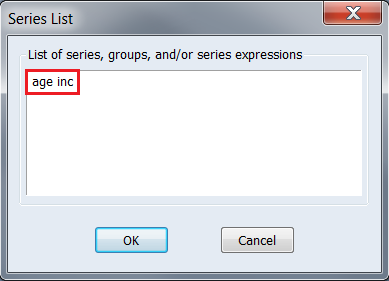
\includegraphics{tute6_q3_9}
\end{figure}
\vspace{-\baselineskip} \centering $(press\ Enter\ to\ execute\ code)$

%%%%%%%%%% TABLE OBJECT %%%%%%%%%%
\begin{table}[H]
	\centering
	\begin{tabular}{lrrrr}
		\multicolumn{3}{l}{Dependent Variable: NETTFA}&\multicolumn{1}{c}{}&\multicolumn{1}{c}{}\\
		\multicolumn{3}{l}{Method: Least Squares}&\multicolumn{1}{c}{}&\multicolumn{1}{c}{}\\
		\multicolumn{3}{l}{Date: 04/09/18   Time: 18:26}&\multicolumn{1}{c}{}&\multicolumn{1}{c}{}\\
		\multicolumn{3}{l}{Sample: 1 9275 IF FSIZE=1}&\multicolumn{1}{c}{}&\multicolumn{1}{c}{}\\
		\multicolumn{3}{l}{Included observations: 2017}&\multicolumn{1}{c}{}&\multicolumn{1}{c}{}\\
		[4.5pt] \hline \\ [-4.5pt]
		\multicolumn{1}{c}{Variable}&\multicolumn{1}{r}{Coefficient}&\multicolumn{1}{r}{Std. Error}&\multicolumn{1}{r}{t-Statistic}&\multicolumn{1}{r}{Prob.}\\
		[4.5pt] \hline \\ [-4.5pt]
		\multicolumn{1}{c}{C}&\multicolumn{1}{r}{$-10.57095$}&\multicolumn{1}{r}{$2.060678$}&\multicolumn{1}{r}{$-5.129843$}&\multicolumn{1}{r}{$0.0000$}\\
		\multicolumn{1}{c}{INC}&\multicolumn{1}{r}{$0.820681$}&\multicolumn{1}{r}{$0.060900$}&\multicolumn{1}{r}{$13.47589$}&\multicolumn{1}{r}{$0.0000$}\\
		[4.5pt] \hline \\ [-4.5pt]
		\multicolumn{1}{l}{R-squared}&\multicolumn{1}{r}{$0.082673$}&\multicolumn{2}{l}{Mean dependent var}&\multicolumn{1}{r}{$13.59498$}\\
		\multicolumn{1}{l}{Adjusted R-squared}&\multicolumn{1}{r}{$0.082218$}&\multicolumn{2}{l}{S.D. dependent var}&\multicolumn{1}{r}{$47.59058$}\\
		\multicolumn{1}{l}{S.E. of regression}&\multicolumn{1}{r}{$45.59223$}&\multicolumn{2}{l}{Akaike info criterion}&\multicolumn{1}{r}{$10.47834$}\\
		\multicolumn{1}{l}{Sum squared resid}&\multicolumn{1}{r}{$4188483.$}&\multicolumn{2}{l}{Schwarz criterion}&\multicolumn{1}{r}{$10.48390$}\\
		\multicolumn{1}{l}{Log likelihood}&\multicolumn{1}{r}{$-10565.41$}&\multicolumn{2}{l}{Hannan-Quinn criter.}&\multicolumn{1}{r}{$10.48038$}\\
		\multicolumn{1}{l}{F-statistic}&\multicolumn{1}{r}{$181.5995$}&\multicolumn{2}{l}{Durbin-Watson stat}&\multicolumn{1}{r}{$1.914495$}\\
		\multicolumn{1}{l}{Prob(F-statistic)}&\multicolumn{1}{r}{$0.000000$}&\multicolumn{1}{c}{}&\multicolumn{1}{c}{}&\multicolumn{1}{c}{}\\
		[4.5pt] \hline \\ [-4.5pt]
	\end{tabular}
	%\caption{Add your caption here.}
	%\label{tab:}
\end{table}
\vspace{-\baselineskip} \centering $\widehat{nettfa} = -\underset{(2.0607)}{10.5710} + \underset{(0.0609)}{0.8207}inc$

\justify \noindent As we can see, the estimated coefficient of $inc$ is now 0.82 which is not that much different from that value of 0.79 obtained in part (b). This implies that there is no significant omitted variable bias for the coefficient on $inc$ after $age$ has been removed.

\noindent If age, which is assumed to belong in the model of net financial wealth, is omitted from the model, $$nettfa = \beta_0 + \beta_1inc + v$$ it is then captured by the error term $v$, $$v = \beta_2age + u$$ If age is also correlated with income, then we will have an omitted variable bias problem i.e. the OLS estimator will be a biased estimator and we will have biased estimates.

\noindent That is, estimating $$nettfa = \beta_0 + \beta_1inc + v$$ with the OLS estimator,  $$\hat{\boldsymbol{\beta}} = (\textit{\textbf{X}}'\textit{\textbf{X}})^{-1}\textit{\textbf{X}}'\textit{\textbf{y}} = \begin{bmatrix}
\hat{\beta}_0 \\
\hat{\beta}_1
\end{bmatrix}$$ will produce biased estimates, $$E(\hat{\boldsymbol{\beta}}) \neq \boldsymbol{\beta}$$

\newpage
\section*{Question 4}
\noindent \textcolor{red}{File $GROWTHED.wf1$ contains observations on GDP per capita (in US dollars) in 2005 and `Average years spent in education in 2005' for 80 countries.}
\begin{figure}[H]
	\centering
	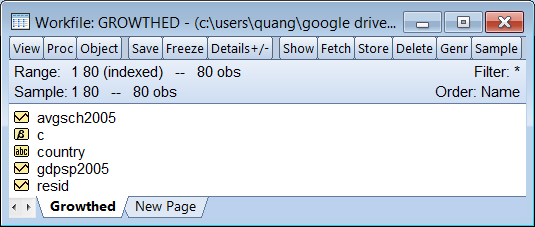
\includegraphics{tute6_q4_1}
\end{figure}
\vspace{-\baselineskip}
\noindent \textcolor{red}{(a) From an economic point of view, what direction would you expect the relationship between GDP and education to have?}

\noindent We would expect countries with higher levels of education on average to be more productive which in turn leads to higher output (income) per worker $\therefore$ a positive correlation between GDP and measures of a country's education.

\noindent \textcolor{red}{(b) Given your conclusion in (a), run the relevant regression, report the estimated model and interpret the estimates for the intercept and slope coefficients.}
$$gdpsp2005 = \beta_0 + \beta_1 avgsch2005 + u$$
\noindent To estimate the model of $gdpsp2005$ from the Command window,
$$Command\ window: ls\ gdpsp2005\ c\ avgsch2005$$
\begin{figure}[H]
	\centering
	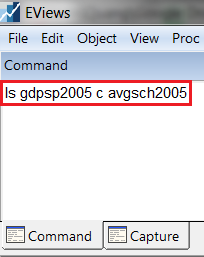
\includegraphics{tute6_q4_2}
\end{figure}
\vspace{-\baselineskip} \centering $(press\ Enter\ to\ execute\ code)$
%%%%%%%%%% TABLE OBJECT %%%%%%%%%%
\begin{table}[H]
	\centering
	\begin{tabular}{lrrrr}
		\multicolumn{4}{l}{Dependent Variable: GDPSP2005}&\multicolumn{1}{c}{}\\
		\multicolumn{3}{l}{Method: Least Squares}&\multicolumn{1}{c}{}&\multicolumn{1}{c}{}\\
		\multicolumn{3}{l}{Date: 04/08/18   Time: 17:30}&\multicolumn{1}{c}{}&\multicolumn{1}{c}{}\\
		\multicolumn{2}{l}{Sample: 1 80}&\multicolumn{1}{c}{}&\multicolumn{1}{c}{}&\multicolumn{1}{c}{}\\
		\multicolumn{3}{l}{Included observations: 80}&\multicolumn{1}{c}{}&\multicolumn{1}{c}{}\\
		[4.5pt] \hline \\ [-4.5pt]
		\multicolumn{1}{c}{Variable}&\multicolumn{1}{r}{Coefficient}&\multicolumn{1}{r}{Std. Error}&\multicolumn{1}{r}{t-Statistic}&\multicolumn{1}{r}{Prob.}\\
		[4.5pt] \hline \\ [-4.5pt]
		\multicolumn{1}{c}{C}&\multicolumn{1}{r}{$-9255.898$}&\multicolumn{1}{r}{$1663.450$}&\multicolumn{1}{r}{$-5.564278$}&\multicolumn{1}{r}{$0.0000$}\\
		\multicolumn{1}{c}{AVGSCH2005}&\multicolumn{1}{r}{$2734.208$}&\multicolumn{1}{r}{$206.1562$}&\multicolumn{1}{r}{$13.26280$}&\multicolumn{1}{r}{$0.0000$}\\
		[4.5pt] \hline \\ [-4.5pt]
		\multicolumn{1}{l}{R-squared}&\multicolumn{1}{r}{$0.692795$}&\multicolumn{2}{l}{Mean dependent var}&\multicolumn{1}{r}{$10976.04$}\\
		\multicolumn{1}{l}{Adjusted R-squared}&\multicolumn{1}{r}{$0.688856$}&\multicolumn{2}{l}{S.D. dependent var}&\multicolumn{1}{r}{$10636.55$}\\
		\multicolumn{1}{l}{S.E. of regression}&\multicolumn{1}{r}{$5933.098$}&\multicolumn{2}{l}{Akaike info criterion}&\multicolumn{1}{r}{$20.23916$}\\
		\multicolumn{1}{l}{Sum squared resid}&\multicolumn{1}{r}{$2.75E+09$}&\multicolumn{2}{l}{Schwarz criterion}&\multicolumn{1}{r}{$20.29871$}\\
		\multicolumn{1}{l}{Log likelihood}&\multicolumn{1}{r}{$-807.5665$}&\multicolumn{2}{l}{Hannan-Quinn criter.}&\multicolumn{1}{r}{$20.26304$}\\
		\multicolumn{1}{l}{F-statistic}&\multicolumn{1}{r}{$175.9018$}&\multicolumn{2}{l}{Durbin-Watson stat}&\multicolumn{1}{r}{$1.540989$}\\
		\multicolumn{1}{l}{Prob(F-statistic)}&\multicolumn{1}{r}{$0.000000$}&\multicolumn{1}{c}{}&\multicolumn{1}{c}{}&\multicolumn{1}{c}{}\\
		[4.5pt] \hline \\ [-4.5pt]
	\end{tabular}
	%\caption{Add your caption here.}
	%\label{tab:}
\end{table}
\vspace{-\baselineskip}
\centering $\widehat{gdpsp2005} = -\underset{(1663.450)}{9255.898} + \underset{(206.1562)}{2734.208}avgsch2005 $
\justify Interpretations of the estimated coefficients:

\noindent $\hat{\beta}_0 = -9255.898$ 

\noindent The model estimates that in a country where people on average have no education ($avgsch2005 = 0$), the level of GDP is per capita is expected to be -\$9,255.90. This result does not make much economic sense.

\noindent $\hat{\beta}_1 = 2734.208$ 

\noindent The model estimates that when average year of education increases by 1 year, the countries level of GDP per capita is expected to increase by \$2,734.208.

\noindent \textcolor{red}{(c) How could you run your regression again to address a strange/meaningless result from your regression in part (b)?}

\noindent We could transformation the independent variable such that the estimated intercept represents GDP per capita for a country whose average level of education is the sample of country's mean average level of education ($\overline{avgsch2005}$), $$newavgsch2005 = avgsch2005 - \overline{avgsch2005}$$

\noindent To generate the variable $newavgsch2005$, $$Genr \to newavgsch2005 = avgsch2005 - @mean(avgsch2005) \to OK$$
\begin{figure}[H]
	\centering
	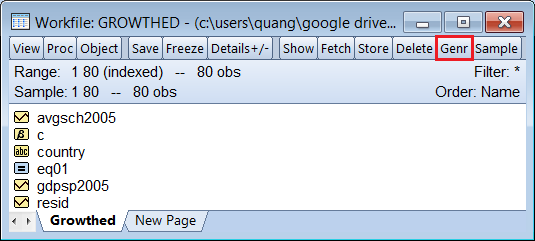
\includegraphics{tute6_q4_3}
\end{figure}
\vspace{-\baselineskip}
\begin{figure}[H]
	\centering
	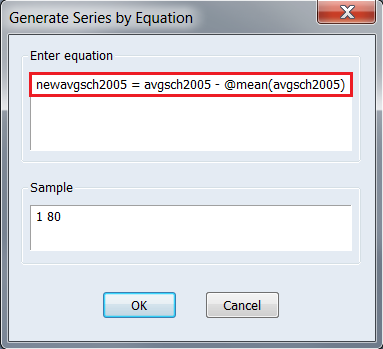
\includegraphics{tute6_q4_4}
\end{figure}
\vspace{-\baselineskip}
\begin{figure}[H]
	\centering
	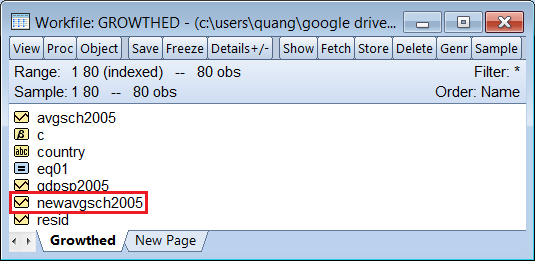
\includegraphics{tute6_q4_5}
\end{figure}
\vspace{-\baselineskip}
\noindent We want to run the following regression: $$gdpsp2005 = \beta_0 + \beta_1 newavgsch2005 + u$$
\noindent to do this from the Command window,
$$Command\ window: ls\ gdpsp2005\ c\ newavgsch2005$$
\begin{figure}[H]
	\centering
	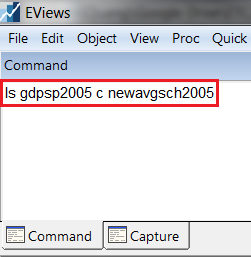
\includegraphics{tute6_q4_6}
\end{figure}
\vspace{-\baselineskip}
%%%%%%%%%% TABLE OBJECT %%%%%%%%%%
\begin{table}[H]
	\centering
	\begin{tabular}{lrrrr}
		\multicolumn{4}{l}{Dependent Variable: GDPSP2005}&\multicolumn{1}{c}{}\\
		\multicolumn{3}{l}{Method: Least Squares}&\multicolumn{1}{c}{}&\multicolumn{1}{c}{}\\
		\multicolumn{3}{l}{Date: 04/08/18   Time: 18:18}&\multicolumn{1}{c}{}&\multicolumn{1}{c}{}\\
		\multicolumn{2}{l}{Sample: 1 80}&\multicolumn{1}{c}{}&\multicolumn{1}{c}{}&\multicolumn{1}{c}{}\\
		\multicolumn{3}{l}{Included observations: 80}&\multicolumn{1}{c}{}&\multicolumn{1}{c}{}\\
		[4.5pt] \hline \\ [-4.5pt]
		\multicolumn{1}{c}{Variable}&\multicolumn{1}{r}{Coefficient}&\multicolumn{1}{r}{Std. Error}&\multicolumn{1}{r}{t-Statistic}&\multicolumn{1}{r}{Prob.}\\
		[4.5pt] \hline \\ [-4.5pt]
		\multicolumn{1}{c}{C}&\multicolumn{1}{r}{$10976.04$}&\multicolumn{1}{r}{$663.3405$}&\multicolumn{1}{r}{$16.54662$}&\multicolumn{1}{r}{$0.0000$}\\
		\multicolumn{1}{c}{NEWAVGSCH2005}&\multicolumn{1}{r}{$2734.208$}&\multicolumn{1}{r}{$206.1562$}&\multicolumn{1}{r}{$13.26280$}&\multicolumn{1}{r}{$0.0000$}\\
		[4.5pt] \hline \\ [-4.5pt]
		\multicolumn{1}{l}{R-squared}&\multicolumn{1}{r}{$0.692795$}&\multicolumn{2}{l}{Mean dependent var}&\multicolumn{1}{r}{$10976.04$}\\
		\multicolumn{1}{l}{Adjusted R-squared}&\multicolumn{1}{r}{$0.688856$}&\multicolumn{2}{l}{S.D. dependent var}&\multicolumn{1}{r}{$10636.55$}\\
		\multicolumn{1}{l}{S.E. of regression}&\multicolumn{1}{r}{$5933.098$}&\multicolumn{2}{l}{Akaike info criterion}&\multicolumn{1}{r}{$20.23916$}\\
		\multicolumn{1}{l}{Sum squared resid}&\multicolumn{1}{r}{$2.75E+09$}&\multicolumn{2}{l}{Schwarz criterion}&\multicolumn{1}{r}{$20.29871$}\\
		\multicolumn{1}{l}{Log likelihood}&\multicolumn{1}{r}{$-807.5665$}&\multicolumn{2}{l}{Hannan-Quinn criter.}&\multicolumn{1}{r}{$20.26304$}\\
		\multicolumn{1}{l}{F-statistic}&\multicolumn{1}{r}{$175.9018$}&\multicolumn{2}{l}{Durbin-Watson stat}&\multicolumn{1}{r}{$1.540989$}\\
		\multicolumn{1}{l}{Prob(F-statistic)}&\multicolumn{1}{r}{$0.000000$}&\multicolumn{1}{c}{}&\multicolumn{1}{c}{}&\multicolumn{1}{c}{}\\
		[4.5pt] \hline \\ [-4.5pt]
	\end{tabular}
	%\caption{Add your caption here.}
	%\label{tab:}
\end{table}
\vspace{-\baselineskip}
\centering $\widehat{gdpsp2005} = \underset{(663.3405)}{10976.04} + \underset{(206.1562)}{2734.208}newavgsch2005 $
\justify The estimated slope coefficient, $\hat{\beta}_1$, remains the same, but the estimated intercept coefficient changes. This estimated intercept coefficient is now interpreted as the estimated level of GDP per capita for a country where the people's average year of education equals to the sample mean average year of education. 

\noindent When, $$avgsch2005 = \overline{avgsch2005}$$ then, \begin{align*}
	newavgsch2005 &= avgsch2005 - \overline{avgsch2005} \\
	&= \overline{avgsch2005} - \overline{avgsch2005} \\
	&= 0
\end{align*}
$$\therefore \widehat{gdpsp2005} = 10976.04 + 2734.208 \times 0 = 10976.04$$
\noindent \textcolor{red}{(d) What is the coefficient of determination in the regression of part (b) and how would you interpret it?} $$R^2 = 69.3\%$$

\noindent Approximately 70\% of the variability in GDP per capita can be explained by the country's average level of education.

\noindent \textcolor{red}{(e) Is there a statistically significant relationship between education and GDP per capita?} 
\begin{figure}[H]
	\centering
	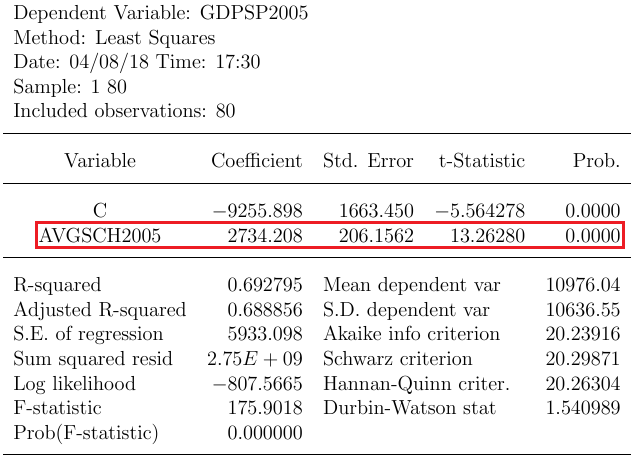
\includegraphics{tute6_q4_7}
\end{figure}
\vspace{-\baselineskip}
\noindent The p-value for a test of statistical significant is reported in the regression output. Here, the p-value is $0.0000$ which is less than $\alpha$ at any reasonable level of significance, therefore we would reject $H_0: \beta_1 = 0$ and conclude that there is sufficient evidence from our sample to suggest that education has a statistically significant effect on GDP per capita.

\noindent \textcolor{red}{(f) What is the 95\% confidence interval for the slope coefficient? Comment on it.} 
$$\hat{\beta}_1 \pm t_{crit} \times se(\hat{\beta}_1)$$
$$\hat{\beta}_1 \pm t_{n-k-1,1-\frac{\alpha}{2}} \times se(\hat{\beta}_1)$$
$$\hat{\beta}_1 \pm t_{78,0.975} \times se(\hat{\beta}_1)$$
\noindent To obtain the 95\% CI of $\beta_1$ in EViews,
$$View \to Coefficient\ diagnostics \to Confidence\ intervals \to 0.95$$
\begin{figure}[H]
	\centering
	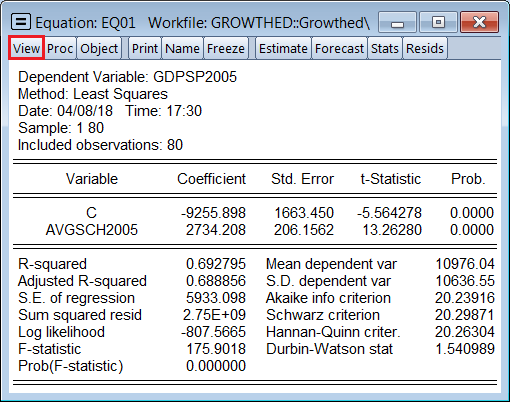
\includegraphics{tute6_q4_8}
\end{figure}
\vspace{-\baselineskip}
\begin{figure}[H]
	\centering
	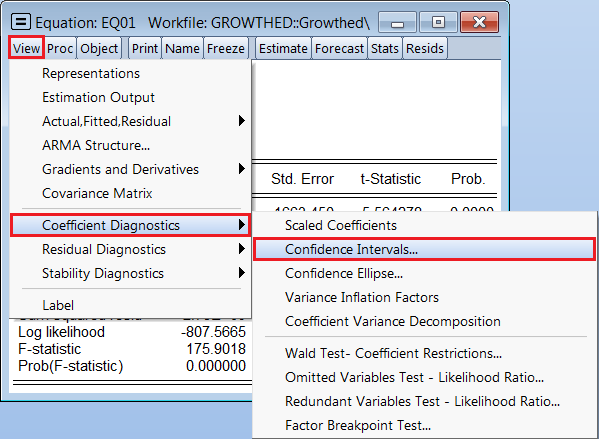
\includegraphics{tute6_q4_9}
\end{figure}
\vspace{-\baselineskip}
\begin{figure}[H]
	\centering
	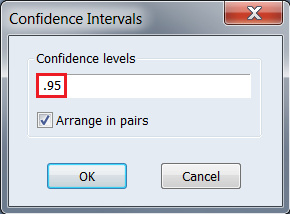
\includegraphics{tute6_q4_10}
\end{figure}
\vspace{-\baselineskip}
%%%%%%%%%% TABLE OBJECT %%%%%%%%%%
\begin{table}[H]
	\centering
	\begin{tabular}{lrrrr}
		\multicolumn{5}{l}{Coefficient Confidence Intervals}\\
		\multicolumn{4}{l}{Date: 04/08/18   Time: 19:07}&\multicolumn{1}{c}{}\\
		\multicolumn{3}{l}{Sample: 1 80}&\multicolumn{1}{c}{}&\multicolumn{1}{c}{}\\
		\multicolumn{4}{l}{Included observations: 80}&\multicolumn{1}{c}{}\\
		[4.5pt] \hline \\ [-4.5pt]
		\multicolumn{1}{c}{}&\multicolumn{1}{c}{}&\multicolumn{1}{c}{}&\multicolumn{2}{c}{95\% CI}\\
		\multicolumn{1}{c}{Variable}&\multicolumn{1}{c}{Coefficient}&\multicolumn{1}{c}{}&\multicolumn{1}{c}{Low}&\multicolumn{1}{c}{High}\\
		[4.5pt] \hline \\ [-4.5pt]
		\multicolumn{1}{c}{C}&\multicolumn{1}{c}{$-9255.898$}&\multicolumn{1}{c}{}&\multicolumn{1}{c}{$-12567.57$}&\multicolumn{1}{c}{$-5944.224$}\\
		\multicolumn{1}{c}{AVGSCH2005}&\multicolumn{1}{c}{$2734.208$}&\multicolumn{1}{c}{}&\multicolumn{1}{c}{$2323.782$}&\multicolumn{1}{c}{$3144.633$}\\
		[4.5pt] \hline \\ [-4.5pt]
	\end{tabular}
	%\caption{Add your caption here.}
	%\label{tab:}
\end{table} \vspace{-\baselineskip}
\centering $(2323.782,3144.633)$
\justify \noindent We are 95\% confident that the true population parameter $\beta_1$ lies between 2323.782 and 3144.633.













\end{document}
